%
% File: chap02.tex
% Author: Hongliang Zhong
%
\let\textcircled=\pgftextcircled
\chapter{Multi-Armed Bandit}
\label{chap:MAB}

\initial{B}andit problems just as we expounded in Chapter~\ref{chap:introduction}, was formally proposed in 1952 by H.Robbins. Generally, this issue could be simplified such a model as below:

A gambling machine with several arms, each of which has an unknown, possibly different distribution of payoffs. The gambler has no idea about which arm with most reward. Considering a sequential decision experiment, the arm $k$ from all arms in an observation being taken from the $i^{th}$ experiment, and the gambler receives a numerical value of this observation as a reward. The observations maybe give him some information useful in the future choices. However,  this observation to obtain information is also to gain rewards. So, the problem for the gambler is how to strike a balance between gaining rewards and obtaining information. 

For example, it is not good to always pull the arm that has performed best in the past, because it may have been that you were just unlucky with the best arm. If you have many trials to go and it only takes a few trials to clarify the matter, you can stand to improve your average gain greatly with only a small investment. Typically in these problems, there is a period of gaining information, following by a period of narrowing down the arms, followed by a period of "profit taking", playing the arm you feel to be the best.

That model is also called ``Multi-Armed Bandit'' (MAB), which is a classical Bandit problem. In this chapter, we focus on describing MAB to understand Bandit problems. The purposes of this chapter is to propose some necessary notions, present some effective strategies,  define and analyze some specific issues. 


\
\
\
\
\
\

%=======

%
% File: chap02.tex section2.1

\let\textcircled=\pgftextcircled

\section{The environment of Multi-Armed Bandit}
\label{sec:environment}

The complexity of Multi-Armed Bandit problems, is not only from the decision-making between Exploration and Exploitation, but also by the wide range of its environments. Each environment to the Multi-Armed Bandit has a different framework. In this section, we address to present the characteristics and performance of Multi-Armed Bandit in each environment, and take the $K$-Armed Bandit as the typical case.
%=========================================================
\subsection{Stationary Bandit}
\label{subsec:stationary}

Stationary Bandit\cite{robbins1952bandit} is the most classical and common bandit problem. The gambler should pick up an arm from the arm setting, where all arms give him a reward for the response. The reward obeys a fixed probability distribution and independent to others arms. 
The $K$-Armed Bandit in stationary environment, can be defined as following setting. The gambler faces to the slot machine with $K$ arms. Where each arm $k$ from the arm set $\mathscr{K} = \{1,\dots, K\}$ is characterized by a distribution $\nu_k$ with its mean reward $\mu_k$ and a variance $\sigma^2_k$, all of these parameters are no changeable. At each round $t \geqslant 1$, the gambler selects an arm $k_t$ and receives a sample drawn from $\nu_{k_t}$ independently of the past. Here, the goal of the gambler is to maximize rewards (minimize regret) or to identify the best arm from all arms by estimating mean rewards after T pulls.

Under T times pull and observation, gambler samples from each arm will be denoted as $T_k = \sum_{t=1}^{T} \1(k = k_t)$. Finally, gambler could estimate the mean of each arm by $\hat{\mu}_{k} = \frac{1}{T_k}\sum_{t=1}^{T_k}X_{k_t,t}$, where $X_{k_t,t}$ denotes the sample received when we pull arm $k$ for the $t^{th}$ time. After $T$ times observation, we find the optimal arm $k^{\ast}$:
\begin{equation}
\label{equa:optarm}
k^{\ast} = \underset{k \in \mathscr{K}}{\text{argmax }} \hat{\mu}_k \text{  and \ \  }
\mu^{\ast} = \underset{k \in \mathscr{K}}{\text{max }} \hat{\mu}_k
\end{equation}

\textbf{Simple Regret}
In the sequel, $\Delta_k = \mu^{\ast}- \hat{\mu}_k$ is the gap between the maximal expected reward and the $k^{th}$ arm of all arms $\mathscr{K}$. And the minimal gap can be noted by $\Delta = \underset{k: \Delta_k>0}{\text{min}} \Delta_k$.
So, the simple regret at round T equals the regret on a one-shot instance for the chosen arm $k_T$, that is,
\begin{equation}
r_T = \mu^{\ast} - \hat{\mu}_{k_T} = \Delta_{k_T}.
\end{equation}

\textbf{Regret}
In the stochastic framework, we define the cumulative regret as:
\begin{equation}
R_T = \sum_{t=1}^{T} (\mu^{\ast}-\hat{\mu}_{k_t})
\end{equation}


\subsection{Adversary Bandit}
\label{subsec:advesary}

Adversary environment\cite{auer2003nonstochastic}, a branch of non-stationary environment, is a challenging problem of the Multi-Armed Bandit. In this environment, the rewards for each step are selected by an adversary rather than the stationary environment where rewards being picked from a fixed distribution. Any method to solve the MAB in adversary environment should recognize that the information between the gambler and the adversary is asymmetry. Similarly to the stationary environment, we define $\mathscr{K} = \{1, \dots, K\}$ be a set of arms, and $\mathscr{T} = \{1,2,\dots,T\}$ denote the sequence of decision epochs by gambler. To compare between the stationary environment and the adversary environment, the difference is the reward distribution of arms. In adversarial environment, the reward distribution $\nu$ is changeable at each epoch $t$ under adversary's control instead of the constant distribution in stationary. From another point of view, adversarial bandit can be seen as a competition between the gambler and an omniscient adversary. 

This issue can be transformed into three step at the iteration $t$:
\begin{itemize}
\item	the adversary choose the reward distributions $\mathbf{\mu_t = (\mu_{1,t},\dots, \mu_{K,t}) \in [0,1]^K }$
\item	the gambler picks one arm $k_t$ with no knowledge of the adversary's choice 
\item	the rewards are assigned $X_{k,t} \sim \mu_{k,t}$
\end{itemize}

\textbf{Regret} who measures the performance of the gambler compared to the performance of the best arm:
\[R_T = \underset{k=1,\dots,K}{\text{max}}\sum_{t=1}^T \mu_{k,t} - \sum_{t=1}^T X_{k_t,t}.\]


\subsection{Contextual Bandit}
\label{subsec:contextual}

Contextual Bandit \cite{agrawal2012thompson,may2012optimistic}, a natural extension of the Multi-Armed Bandit problem, is obtained by associating side information with each arm. Based on this side information, or context, some applications could be modeled naturally as Multi-Armed Bandit problem with context information, so it also named as Bandit with side information. As it is closely related to work in machine learning on supervised learning and reinforcement learning. In order to facilitate the presentation in Chapter~\ref{chap:BF}, the definitions of Contextual Bandit, will be referred to some notations in supervised learning.

For contextual bandit, there is a distribution $\mathbb{P}$ over $(x, r_1, r_2,\dots,r_K)$. On each round $t\in \mathscr{T}=\{1, 2, \dots\}$, the gambler receives a sample $(x_t, r_{t,1},r_{t,2},\dots, r_{t,K})$ drawn from $\mathbb{P}$ and makes decision $\hy \in \mathscr{Y}$ by observing the set of arms $\mathscr{Y} = \{1,\dots,K\}$ with side information a feature vector $\mathbf{x}_{t,y_t} \in \mathscr{X}$. Where $y_t$ is the optimal arm for $x_t$, but gambler do not know this. With the chosen arm $\hy$, gambler receives a  reward $r_{(x_t,\hy)}$. We should emphasize that the reward is only observed for the arm chosen . 

After $\mathscr{T}$ sequence, all rewards for gambler is defined as $\sum_{t=1}^{T}r_{(x_t,\hy)}$. Similarly referring to the stationary setting, we define the regret by the notations above:
\[R(T) = \mathbb{E}[\sum_{t=1}^{T}r_{(x_t,y_t)}] - \mathbb{E}[\sum_{t=1}^T r_{(x_t,\hy)}].\]

Contextual bandits naturally arise in many applications. For example, online recommendation systems, advertisement push, personalized search etc.

\subsection{Linear Bandit}
\label{subsec:linear}
Linear Bandit problem\cite{abbasi2011improved, carpentier2012bandit} is also a sequential decision-making problem as same as other bandit problem, where in each step, the gambler has to choose an arm from the arms set. As a response, the gambler receives a stochastic reward, expected value of which is an unknown linear function of the chosen arm.

Here, we present formally the process of Linear Bandit problem. On round $t$, gambler is given the arms set $\mathscr{K} \subseteq \mathbb{R}^d$. From which he should select an arm $k_t\in\mathbb{R}^d$. Then, the gambler observes a reward $r_t = <k_t,\theta> + \eta_t$ where $\theta\in \mathbb{R}^d$ is an unknown parameter and $\eta_t$ is a random noise satisfying the condition $\mathbb{E}[\eta_t| k_{1:t}, \eta_{1:t-1}] = 0 $. 

As other bandit problems, the goal of this problem is to maximize the cumulative reward $R = \sum_{t=1}^T <k_t,\theta>$ over all round $T$. Obviously, the gambler would choose the optimal arm $k^{\ast} = \underset{k\in\mathscr{K}}{\text{argmax }}<k,\theta>$ with the knowledge of $\theta$. As a result, the regret of linear bandit problem, can be formally denoted as 
\[R = \left(\sum_{t=1}^T <k_t^{\ast},\theta>\right) - \left(\sum_{t=1}^T <k_t,\theta>\right) = \sum_{t=1}^T <k_t^{\ast}-k_t, \theta>\].


\section{Gittins index}
\label{sec:gittins}

Multi-Armed Bandit is concerned with sequential decision. The definition can be found at the head of this chapter. In this section, we focus on his optimal decision process.  Someone treat MAB problem as a Markov Decision Process (MDP). However, there is no approach can scale well it on considering the curse of dimensionality by the number of bandit process. In that situation, Gittins and Jones \cite{gittins1974dynamic} show that the problem can be reduced to solve $K$ $1$-dimensional problems from the $K$-dimensional Markov Decision Process  with the state space $\prod_{k=1}^{K}X(k)$, where $X(k) = (x(k,1),x(k,2),\dots)$ present the state of arm $k$. So that, $K$-armed bandit returns denoted by 
\[
\begin{split}
 \text{arm }1: x(1,1),x(1,2),\dots, x(1,t), \dots\\
 \text{arm }2: x(2,1),x(2,2),\dots, x(2,t), \dots \\
\dots \\
 \text{arm }K: x(K,1),x(K,2),\dots, x(K,t), \dots \\
\end{split}
\]
For each arm $k$, to compute
\begin{equation}
\label{equa:gittins}
\mathscr{G}_k(X(k)) = \underset{\tau >0}{\text{sup}} \frac{\mathbb{E}[\sum_{t=0}^{\tau-1}\beta^t r_k(x(k,t))|x(k,0) = x(k)]}{\mathbb{E}[\sum_{t=0}^{\tau-1}\beta^t|x(k,0)=x(k)]}
\end{equation}
where $\tau$ is a stopping time constrained and $\mathscr{G}_k$ is the value of the Gittins index for arm $k$. The stopping time $\tau$ represents the first time at which the index for this arm may be optimal no more. For its index neither greater than the initial value. By the way, the decision rule is then to simple arm $k_t$, which can be computed by the format $k_t = \underset{k\in \mathscr{K}}{\text{argmax }} \mathscr{G}_k(X(k))$. 

\begin{theo}{Gittins Index Theorem}
\label{theo:gittins}
The problem posed by a simple family of alternative bandit processes, as setup above, is solved by always continuing the process having the greatest \textbf{Gittins Index}, which is defined as Function~\ref{equa:gittins}.
\end{theo}
To this theorem, there are various proofs have been given, the original proof is proposed by Gittins and Jones\cite{gittins1974dynamic}, and a later proof by Gittins \cite{gittins1979bandit} relied on an interchange argument. Further simplified by \cite{varaiya1983extension, tsitsiklis1994short}. More details about the proofs can be referred in their papers.

Gittins Index characterized the optimal strategy as Theorem~\ref{theo:gittins}, an equivalent interpretation of the Gittins Index strategy is the following:
\begin{itemize}
\item	Select the arm with the highest Gittins Index $\mathscr{G}_k(X(k))$ and play it until its optimal stopping time and repeat.
\end{itemize}
Thus, an alternative way to implement the optimal way is to compute the value of Gittins index $\mathscr{G}_k(X(k))$ and the corresponding stopping time $\tau$ for the current state $x(k,t)$. 

Scott \cite{scott2010modern} points out two further concerns that the Gittinx Index strategy  is only optimal for the process in which arms are independent and can be far from optimal when this is not the case. 


%
% File: chap02.tex section 2.2 
% Author: Hongliang Zhong
%
\let\textcircled=\pgftextcircled
\section{The strategy of trade-off}
\label{sec:tradeoff}

The synopsis of Bandit problems have been introduced in Section~\ref{sec:environment}. From this synopsis, we get the difficult point of Bandit problem is to keep a balance between Exploration and Exploitation. So that, it becomes very important to trade off between to exploit from the past knowledge to focus on the arms that seems to yield the highest rewards and to explore further the other arms to identify that better which may be the actual global optimal. 

The easiest way to solve this problem, is to select randomly. However, this way mainly relies on luck. So it is not reliable. Another simple way is called ``Naive Sampling'' approach. At early times, it samples each arm by same number, and then measure the results on comparing these samples. After that, an optimal empirical solution has been shown. But this approach also has a problem, that is, if the initial number of samples is too small, the confidence will be low; if the initial number are huge enough, will waste the cost. Therefore, in this section, we will introduce some effective strategies to solve bandit problems.
\
\
\
\
\
\


%=======

\subsection{Thompson Sampling}
\label{subsec:thompson}

Thompson Sampling \cite{thompson1933likelihood}, a randomized algorithm based on Bayesian ideas, is one of oldest heuristic principle  for Bandit problems. Recently, it has been considered having better empirical performance compared to the state-of-the-art methods after several studies demonstrated \cite{chapelle2011empirical,agrawal2011analysis,agrawal2012thompson}.

The origins of Thompson Sampling has been introduced in Chapter~\ref{chap:introduction}, is from the procedure's inventor  William R. Thompson. Thompson was interested in the general problem of research planning. He was concerned with being able to utilize a small numbers of observations in order to steer actions taken before more data could be collected.
This was in the context of a perceived objection to argument based on small numbers of observations at the time. Thompson posed his problem in terms of deciding between two treatments in a clinical trial. One of the treatments would  be administered to a patient in the trials population and the effect could be observed. These observations could then be incorporated into the decision-making process to improve the odds of the most effective treatment being administered to further patients.

For Bandit problems, this randomized strategy will choose an arm with some probability which matches the probability that the arm is in fact the optimal arm, by giving all past observations of all arm pulls. More reasonable for this randomized chosen is to define the probability that an arm is the best is a Bayesian estimate. 

Being more precise, let $\theta$  be a parameter vector on behavior of a bandit problem. The probability that an arm $k$ is optimal, 
\begin{equation}
P(K=k^{\ast}) = \int_{\theta}\mathds{1}(K=k^{\ast}|\theta)P(\theta)\mathrm{d}\theta.
\end{equation}

An arm is thus pulled with the probability $P(K=k^{\ast})$. This Sampling way could be viewed as forming a decision based on one-step Monte-Carlo Sample by estimating the probability of an arm being the best.

The integral above may not have a closed form solution. The integral may be approximated by quadrature. However, this is undesirable as the running cost of each decision will depend on the difficulty of the multi-armed bandit problem. The insight used in Thompson Sampling is that instead we can sample from a distribution defined by $P(K=k^{\ast})$ by simply first sampling a candidate $\theta$ from the distribution $P(\theta)$. 
Given a candidate $\theta$ we can then just pull the arm that is best given this candidate $(\1(K=k^{\ast}|\theta))$. $P(\theta)$ is initially specified as  a prior and then later inferred using Bayes rule as rewards from arm pulls are observed . The general Thompson Sampling algorithm for a $K$-armed bandit is therefore described as following
%!ALGORITHM-----------------------------
\begin{algo}[Thompson Sampling]
\label{algo:thompson1}
\begin{algorithmic}
\STATE $\ \ $
\STATE Initialise $P_{(\mu_1,\dots,\mu_K)}$, the prior belief of the mean payoffs of arms $1,\dots,K$. 
\STATE Let $H_t$ be the history of action, reward pairs $(r_{\tau}, k_{\tau})$ for $1\leqslant \tau \leqslant t$, $H_1 = \{ \}$
\FOR {each round t = 1,2,\dots, T}
	\STATE Sample $\theta_i,\dots,\theta_K \sim P(\mu_1,\dots,\mu_K|H_t)$.
    \STATE Pull arm $k_t = argmax_{k \in \{1,\dots,K\}} \theta_k$
    \STATE Receive reward $\mathds{1}_{r(k_t)=1}$
	\STATE Let $H_{t+1} = H_t \cup (k_t,\mathds{1}_{r(k_t)=1})$.
\ENDFOR
\end{algorithmic}
\end{algo}
%!----------------------------------------


\textbf{Optimism in Thompson Sampling}
There is a question, what is the tradeoff between exploration and exploitation for Thompson Sampling. May \cite{may2012optimistic} tried to separate the two aspects of this algorithm. To do this, he defined the exploitative value of an arm to be the expected payoff of an arm conditioned on the rewards. The estimated value of an arm could be seen as the value of the sampling drawn from the posterioi distribution for the arm. With these, the exploratory value of an arm could then by found by subtracting the exploitative value from the estimated sample value. They observed that this exploratory value could sometimes be negative and so there would be no value from an exploration point of view to pull the arm. The exploratory value of an arm is only negative when the sample estimate drawn from the posterior is less than the exploitative value of the arm. 

In Thompson Sampling, samples are drawn from the posterior distribution of each arm, that is $\theta_k(t)\sim P_{(\mu_k)}$. Instead, Optimistic Thompson Sampling drawn samples such that $\theta_k(t) = max(\mathbb{E}[\mu_k],s_k(t))$ where $s_k(t)\sim P_{(\mu_k)}$. In other words if a sample from the posterior distributions is less than the mean of the distribution, then we take the sample to be then mean. This ensures that the exploratory value of an action is always positive. In Appendix Algorithm~\ref{algo:thompson3} more formally presents the algorithm specifically for the Bernoulli bandit. May\cite{may2012optimistic} observed empirically that Optimistic Thompson Sampling performed better than standard Thompson Sampling.(See in Appendix~\ref{algo:thompson3})

\subsection{Boltzmann Exploration (Softmax)}
\label{subsec:softmax}
This section, is about  Boltzmann Exploration (also named  Softmax), which is based on the axiom of choice \cite{luce1959individual} and pick each arm with a probability that is proportional to its average  behavior. Arms with greater empirical means could be therefore picked with higher probability. Softmax  selects arms by using a Boltzmann distribution. Given initial empirical means $\hat{\mu}_1(0),\dots,\hat{\mu}_K(0)$,
\begin{equation}
\label{equa:boltzmann}
p_k(t+1) = \frac{\exp{\hat{\mu}_k(t)/\tau}}{\sum_{i=1}^{K}\exp{\hat{\mu}_i(t)/\tau}}, \text{where } k\in \{1,\dots,K\}
\end{equation}

Softmax may depend on the task and on human factors by the only parameter $\tau$. Where $\tau$ is a temperature parameter, controlling the randomness of the choice. When $\tau = 0$, Boltzmann Exploration acts like pure greedy. On contrast, $\tau$ tends to infinity, the algorithms picks arms uniformly at random. Most people find it easier to set the $\tau$ requires knowledge of the likely action values and of powers of $e$.

%!ALGORITHM-----------------------------
%!--------------------------------------
\begin{algo}[SoftMax]
%\caption{SoftMax}
\label{algo:softmax1}
\begin{algorithmic}
\STATE {\ }
\STATE Parameter: real number $\tau > 0$
\STATE Initialization: Set $\hat{\mu}_k(0) = 0$ for $\forall k \in [1,\dots,K]$
\FOR {each round t = 1,2,\dots, T}
	\STATE Sample arms $i$ according to the distribution $P(t)$, where
    \[P_k(t) = \frac{\exp \left(\hat{\mu}_k(t-1)/\tau\right)}{\sum_{i=1}^{K} \exp \left(\hat{\mu}_i(t-1)/\tau\right)}\]
    \STATE Receive the reward $r_{k_t}$, here $k_t$ is the sampled arm for instant t 
    \STATE Let $\hat{\mu}_{k}(t) = \sum_t r_{k,t}/ \sum_t \1_{k = k_t,t}$
\ENDFOR
\end{algorithmic}
\end{algo}
%!----------------------------------------

The Softmax strategy could be modified in the same way as the $\epsilon$-greedy strategy in Section~\ref{subsec:greedy} into decreasing Softmax where the temperature decreases with the number of rounds played. The decreasing Softmax is identical to the Softmax but with a temperature $\tau_t = \tau_0/t$ that depends on the index $t$ of the current round. The choice of the value of $\tau_0$ is left to the user. The decreasing Softmax is analyzed by Cesa-Bianchi \cite{cesa1998finite} with the Softmix algorithm. 

A more complicated variant of the Softmax algorithm, the EXP3 ``(see in Appendix~\ref{algo:softmax2})exponential weight algorithm for Exploration/Exploitation'' is introduced in \cite{auer1995gambling}. The probability of choosing the arm $k$ at the round of index $t$ is defined by 
\begin{equation}
P_k(t) = (1-\gamma)\frac{w_k(t)}{\sum_{i=1}^{K}w_i(t)}+\frac{\gamma}{K}
\end{equation}
where $w_i(t+1) = w_i(t) exp\left(\gamma\frac{r_i(t)}{P_i(t)K}\right)$,
if the arm $i$ has been pulled at time t with $r_i(t)$ being the observed reward,
$w_i(t+1) = w_i(t)$ otherwise. The choice of the value of the parameter $\gamma\in (0,1]$ is left to the user.
The main idea is to divide the actual gain $r_i(t)$ by the probability $P_i(t)$ that the action was chosen. For a modified version of EXP3, with $\gamma$ decreasing over time, it is shown by \cite{auer2003nonstochastic}, that a regret of $O(\sqrt{KT\log{K}})$ is achieved.

\subsection{Upper Confidence Bound}
\label{subsec:ucb}
Upper Confidence Bound (UCB) was proposed by Lai \cite{lai1985asymptotically}, to deal with the Exploration and Exploitation dilemma in the Multi-Armed Bandit problem by using Upper Confidence Values. Most strategy for trading off Exploration and Exploitation, they have one weakness: they do not keep track of how much they know about any of options available to them. They pay much more attention only to how much reward they got. This means that they will under-explore options whose initial experiences were not rewarding, even though they don't have enough data to be confident about those options. But UCB can do better that pays attention to not only what it knows, but also how much it knows. 

For example, in stochastic Multi-Armed Bandit problem, gambler has to choose in trials $t\in \{1,2,\dots,T\}$ an arm from a given set of arms $\mathscr{K} = \{1,\dots,K\}$. 
In each trial $t$ the gambler obtains random reward $r_{k,t}\in \{0,1\}$ for choosing arm $k$. 
It is assumed that for each arm $k$ the random reward $r_{k,t}$ is independent and identically distributed random variables with mean $\mu_k$ which is unknown. 
Further, it is assumed that the rewards $r_{k,t}$ and $r_{k',t'}$ for distinct arms $k,k'$ are independent for all $k\neq k' \in \mathscr{K}$ and all $t, t' \in \mathscr{T}$.
 
The gambler's aim is to compete with the arm giving highest mean reward $\mu^{\ast}:= max_{k\in \mathscr{K}} \mu_k$. The arm with the best estimate $\hat{\mu}^{\ast}$ so far serves as a creteria, and other arms are played only if the upper bound of a suitable confidence interval is at least $\hat{\mu}^{\ast}$. That way, within $T$ trials each suboptimal arm can be shown to be played at most $\left(\frac{1}{D_{KL}}+o(1)\right)\log{T}$ times in expectation, where $D_{KL}$ measures the distance between the reward distributions of the optimal and the suboptimal arm by the Kellback-Leibler divergence, and $o(1) \rightarrow 0$ as $T \rightarrow \infty$. This bound was also shown to be asymptotically optimal\cite{lai1985asymptotically}.

Auer \cite{auer2003using} introduced the simple, yet efficient UCB algorithm, that is also based on the ideas of Lai's. After playing each arm once for initialization, UCB chooses at trial $t$ the arm $k$ that maximizes
\begin{equation}
\label{equa:UCB}
\hat{\mu}_k+\sqrt{\frac{2\log{t}}{n_k}}
\end{equation},
where $\hat{\mu}_k$ is the average reward obtained from arm $k$, and $n_k$ is the number of times arm $k$ has been played up to trial $t$. The value in Equation~\ref{equa:UCB} can be interpreted as the Upper Bound of a confidence interval, so that the true mean reward of each arm $k$ with high probability is below this upper confidence bound.

In particular, the upper confidence value of the optimal arm will be higher than the true optimal mean reward $\mu^{\ast}$ with high probability. Consequently, as soon as a suboptimal arm $k$ has been played sufficiently often so that the length of the confidence interval $\sqrt{\frac{2\log{t}}{n_k}}$ is small enough to guarantee that
\[\hat{\mu}_k+\sqrt{\frac{2\log{t}}{n_k}} < \mu^{\ast}
\],
arm $k$ will not be played anymore with high probability. As it also holds that with high probability
\[\hat{\mu}_k<\mu_k+\sqrt{\frac{2\log{t}}{n_k}}\],
arm $k$ is not played as soon as 
\[2\sqrt{\frac{2\log{t}}{n_k}}<\mu^{\ast}-\mu_k\],
that is, as soon as arm $k$ has been played
\[\left \lceil \frac{8\log{t}}{(r^{\ast}-r_k)^2} \right \rceil\]
times. This informal argument can be made stringent to show that each suboptimal arm $k$ in expectation will not be played more often than $\frac{\log{T}}{\Delta_k^2}$ times within $T$ trials, 
where $\Delta_k:=\mu^{\ast}-\mu_k$ is the distance between the optimal mean reward and $\mu_k$.

%!ALGORITHM-----------------------------
%!--------------------------------------
\begin{algo}[Improved UCB algorithm]
%\caption{Improved UCB algorithm}
\label{algo:UCB1}
\begin{algorithmic}
\STATE {\ }
\STATE Set arms $\mathscr{K}= \{1,\dots,K\}$, all playing times $\mathscr{T} = 1,2, \dots, T$
\STATE Initialization: Set $\tilde{\Delta}_0:=1$, and $B_0:=\mathscr{K}$.
\FOR {each round $t = 1,2,\dots, \left \lfloor \frac{1}{2}\log{\frac{T}{e}} \right \rfloor$ }
	\STATE Select arm: if $|B_m|>1$, choose each arm in $B_m$ until the total number of times it has been chosen is $n_m:= \left \lceil \frac{2\log{T\tilde{\Delta}^2_m}}{\tilde{\Delta}^2_m} \right \rceil$. Otherwise choose the single $B_m$ until step $T$ is reached.
	\STATE Eliminate arm: Delete all arms $i$ from $B_m$ for which
    \[ \left\{ \hat{\mu}_i+\sqrt{\frac{\log{T\tilde{\Delta}^2_m}}{2n_m}} \right\} < \text{max}_{j\in B} \left\{ \hat{\mu}_j - \sqrt{\frac{\log{T\tilde{\Delta}^2_m}}{2n_m}}\right\} \] in order to obtain $B_{m+1}$. Here $\hat{\mu}_j$ is the average reward obtained from arm $j$.
    \STATE	Reset $\tilde{\Delta}_m$: Set $\tilde{\Delta}_{m+1} = \frac{\tilde{\Delta}_m}{2}$
\ENDFOR
\end{algorithmic}
\end{algo}
%!----------------------------------------

In \cite{auer2010ucb}, Auer proposed an improved UCB algorithm (shown in Algorithm~\ref{algo:UCB1}). In this improved model, gambler can access to the values $\Delta_k$, one could directly modify the confidence intervals of UCB as given \cite{agrawal1995sample} to $\sqrt{\frac{2\log{t\Delta_k^2}}{n_k}}$, and the proof of the claimed regret bound would be straightforward.

However, since the $\Delta_k$ is unknown to the learner, the modified algorithm shown in Algorithm~\ref{algo:UCB1} guesses the values $\Delta_k$ by a value $\tilde{\Delta}$, which is initialized to 1 and halved each time the confidence intervals become shorter than $\tilde{\Delta}$. Note that compared to the original UCB algorithm the confidence intervals are shorter, in particular for arms with high estimated reward. Unlike the original UCB algorithm, our modification eliminates arms that perform bad. As the analysis will show, each suboptimal arm is eliminated as soon as $\tilde{\Delta}<\frac{\Delta_k}{2}$, provided that the confidence intervals hold. Similar arm elimination algorithms were already proposed in \cite{even2006action}. 

\subsection{Epsilon-Greedy}
\label{subsec:greedy}

In this section, we are going to introduce a simple algorithm for trading off exploration and exploitation. This strategy is called $\epsilon$-Greedy\cite{Sutton98} (shown in Appendix~\ref{algo:epsilon}). In computer science, a greedy algorithm is an algorithm that always takes whatever action seems best at the present moment, even when that decision might lead to bad long term consequences. The $\epsilon$-greedy algorithm is almost a greedy algorithm because it generally exploits the best available option, but also have some chance to explore the other available options. 
\begin{figure}[!h]
\centering{
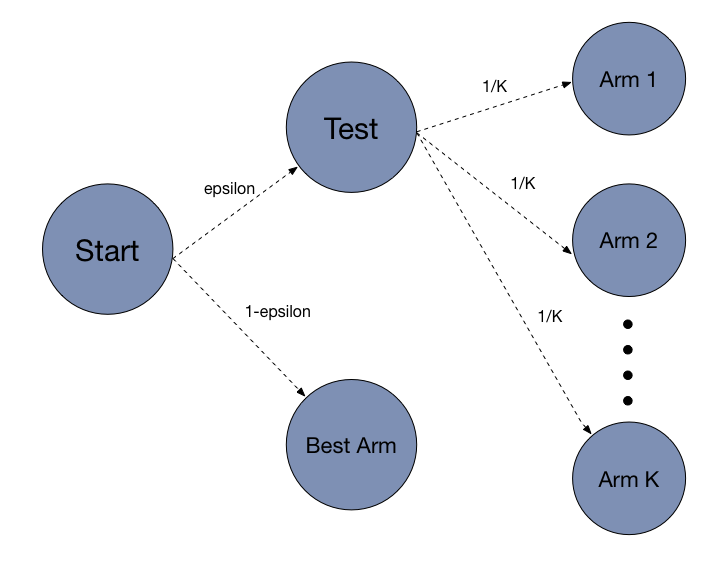
\includegraphics[scale = 0.4]{chapters/chapter02/fig02/epsilongreedy.png}}
\caption{the mechanism of epsilon-greedy}
\label{fig:epsilon}
\end{figure}

Let's be more concrete to the mechanism of $\epsilon$-greedy algorithm. It works by randomly oscillating between the purely randomized experimentation and instinct to maximize profits. The $\epsilon$-greedy is one of the easiest bandit algorithms to understand because it tries to be fair to the two opposite goals of exploration and exploitation by using a mechanism (see the Figure~\ref{fig:epsilon}). Take a simple example to understand easily: it is just like flipping a coin. If you flip a coin and it comes up heads, you should explore for a moment. But if the coin comes up tails, you should exploit.

The formal process as follows,
\begin{itemize}
\item Firstly, pick a parameter $\epsilon \in [0,1]$, 
\item Then, at each step greedily play the object with highest empirical mean reward with probability $1-\epsilon$ and play a random arm with probability $\epsilon$. 
\item Receives the reward from the arm chosen
\item Finally, update the empirical means of each arm.
\end{itemize}

%!ALGORITHM-----------------------------
%!--------------------------------------
\begin{algo}[$\epsilon$-Greedy]
%\caption{$\epsilon$-Greedy}
\label{algo:epsilon}
\begin{algorithmic}
\STATE {\ }
\STATE Initialise $P_{(\mu_1,\dots,\mu_K)}$, the prior belif of the mean payoffs of arms $1,\dots,K$. 
\FOR {each round t = 1,2,\dots, T}
	\STATE Pull arm $k_t = \begin{cases}
    \text{argmax}_{k\in \{1,\dots,K\}} P_{(\mu_k)} & \text{with probability}\ \epsilon \\
    \text{select randomly} & \text{with probability}\ 1-\epsilon
    \end{cases}$ 
    \STATE Receive reward $r_{(k_t)}$
	\STATE Update $\mu_{k_t}$ by the reward $r_{(k_t)}$.
\ENDFOR
\end{algorithmic}
\end{algo}
%!----------------------------------------

Auer~\cite{Auer02Finite} has proven that, if $\epsilon$ is allowed to be a certain function $\epsilon_t$ following the current time step $t$, namely $\epsilon_t = K/(d^2t)$, then the regret grows logarithmically like $(K \log{T}/d^2)$, provided $d$ less than the number of objects with minimum regret . While this bound has a suboptimal dependence on $d$. In Auer's~\cite{Auer02Finite} same paper, it show that this algorithm performs well in practice, but the performance degrades quickly if $d$ is not chosen as a tight lower bound.

Compared to other more complex methods, $\epsilon$-greedy is often hard to beat and reported to be often the method of the first choice as stated . In practice, however, a drawback of $\epsilon$-greedy is that it is unclear which setting of $\epsilon$ leads to good results for a given learning problem. For this reason, the experimenter has to rigorously hand tune $\epsilon$ for obtaining good results, which can be a very time-consuming task in practice depending on the complexity of the target application.

One method that aims at overcoming the above mentioned limitation of $\epsilon$-greedy is ``Value-Difference Based Exploration''(VDBE)\cite{tokic2010adaptive}. In contrast to pure $\epsilon$-greedy, VDBE adapts a state-dependent exploration-probability. The basic idea of VDBE is to extend the $\epsilon$-greedy method by controlling a state-dependent exploration probability, $\epsilon(s)$, in dependence of the value-function error instead of manual tuning. The desired behavior is to have the agent more explorative in situations when the knowledge about the environment is uncertain, i.e. at the beginning of the learning process, which is recognized as large changes in the value function. On the other hand, the exploration rate should be reduced as the agent's knowledge becomes certain about the environment, which can be recognized as very small or no changes in the value function. 


\section{Regret Lower bound for the stochastic Multi-Armed Bandit problems}
\label{sec:lowerbound}

Lai and Robbins \cite{lai1985asymptotically} provided asymptotic lower bounds of the expected regret for the stochastic Multi-Armed Bandit problem. In their work, it shows that $R(T) = o(T^a)$ can applies to any strategy for MAB, for all $a>0$ as $T\rightarrow \infty$. 

Kaufmann et al.\cite{Kaufmann12} call this condition strongly consistent, since that $\text{lim}_{T\rightarrow \infty} \E[S(T)] /T =\mu_{\text{max}}$. When the reward distribution are Bernoulli, for arms $i,j$, their reward average $\mu_i,\mu_j \in [0,1]$ To define the Kullback-Leibler divergence between two Bernoulli distributions with parameters $\mu_i$ and $\mu_j$
\[D_{KL}(\mu_i,\mu_j) = \mu_i\ln{\frac{\mu_i}{\mu_j}}+(1-\mu_i)\ln{\frac{1-\mu_i}{1-\mu_j}}
\] 

The Theorem of asymptotic lower bounds states that 
\begin{theo}{Distribution-dependent lower bound}
\label{theo:lowerbound}
Consider a strategy that satisfies $R(T) = o(T^a)$ for any set of Bernoulli reward distributions, any arm $k$ with $\Delta_k = \mu^{\ast}-\mu_k >0$, and any $a>0$. Then, for any set of Bernoulli reward distributions the following holds
\begin{equation}
\label{equal:lowerbound}
\underset{T\rightarrow\infty}{\text{lim}} \text{inf}\frac{R(T)}{\ln{T}} \geqslant \sum_{k\in \mathscr{K}: \Delta_k>0} \frac{\Delta_k}{D_{KL}(\mu_k,\mu^{\ast})}
\end{equation}
\end{theo}
Let $N_{k,T}$ be the number of times the strategy pulled arm $k$ up to time $T$, the bound can be written as, 
\[\underset{T\rightarrow \infty}{\text{lim}}\text{inf} \frac{\sum_{k\in K}\E[N_{k,T}(\mu_{max}-\mu_k)]}{\ln{T}}
\]

They call any strategy that meets this lower bound with equality asymptotically efficient. It's also useful to note that for a strategy that satisfies
\[\underset{T\rightarrow \infty}{\text{lim}}\frac{\E[N_{k,T}]}{\ln{T}} \geqslant \frac{1}{D_{KL}(K,\mu_{max})},\]
with equality for all $k\in K$ then refer to the Equation~\ref{equal:lowerbound} satisfy with equality and the strategy is asymptotically optimal.

\section{Pure Exploration and Best Armed Identification in Multi-Armed Bandit}
\label{sec:bestarm}

Bubeck \cite{bubeck2009pure, bubeck2011pure} and Chen \cite{chen2014combinatorial} proposed the same problem that the gambler may sample arms under a given number of times $T$ which may be not necessary to know in advance, and be asked to output an arm recommended. They advocate to evaluate the performance of gambler by the simple regret (refer the section~\ref{subsec:stationary}). The distinguish from the classical MAB's modeling is to separate the exploration phase and the exploitation phase. This is the pure exploration problem. Its process is shown as the following modeling,
\begin{itemize}
\item	Definir the number of rounds $T$ and number of arms $K$ to gambler;
\item	Parameters the reward distribution $\nu_1,\dots,\nu_K$ of the arms which is unknown to ganbler;
\item	Repeat that gambler chooses an arm $k_t \in \mathscr{K}$ and receives the reward $r_{(k_t,t)}$ drawn from $\nu_{k_t}$ and independently from the past;
\item Finally, the gambler outputs the recommendation $k^{\ast}$ arm from the arm set $\mathscr{K}$.
\end{itemize}

The pure exploration problem is about the design of strategies who makes the best use of the limited budget in order to optimize the performance and identifier their best choice of a decision-making task. Audibert \cite{audibert2010best} proposed two algorithms to address this problem: UCB-E and Successive Rejects. The former is a highly exploring strategy based on Upper Confidence Bounds, the latter is a parameter-free method based on propressively rejecting the arms which seem to be suboptimal. Audibert shows that these two algorithms are essentially optimal since the regret decrease exponentially at a rate which up to a logarithmic factor.

\subsection*{UCB-E algorithm} 
This algorithm is the highly exploring policy based on Upper Confidence bounds(UCB-E). When the exploration parameter $a$ (shown in Appendix~\ref{algo:ucbe}) is taken of order $\log{T}$, the algorithm essentially corresponds to the UCB1 algorithm introduced in \cite{auer2010ucb}. And its cumulative regret is of order $\log{T}$. \cite{bubeck2009pure} have shown that algorithms having at most logarithmic cumulative regret, have at least a (non-cumulative) regret of order $T^{-\gamma}$ for some $\gamma > 0$. So taking the parameter $a$ of order $\log{T}$ is not befitting to reach exponentially small probability of error. It should take $a$ as linear in $T$ can explore much more than ever. The theorem below cited from \cite{audibert2010best}

\begin{theo}
\label{theo:ucbe}
If UCB-E is run with parameter $0 < a \leqslant \frac{25}{36} \frac{T-K}{H_1}$, then it satisfies
\begin{equation}
e_T \leqslant 2TK\exp{-\frac{2a}{25}}.
\end{equation}
In particular for $a=\frac{25}{36}\frac{T-K}{H_1}$, we have $e_T \leqslant 2TK\exp{-\frac{T-K}{18H_1}}$
\end{theo}

Where $e_T$ denote the probabiity of error that the recommendation $ k_T$ equals to the optimal arm $k^{\ast}$ and $H_1$ denotes a quantity $H_1 = \sum_{k=1}^{K}\frac{1}{\Delta_k^2}$ (the definition of $\Delta_k$ in Section~\ref{subsec:stationary}). Theorem~\ref{theo:ucbe} shows that the probability of error of UCB-E is at most of order $\exp{-a}$ for $a\geqslant \log{T}$. 

In view of the parameter $a$ if $a \leqslant \frac{25}{36}\frac{T-K}{H_1}$, it can be essentially said: the more it explores, the smaller the regret is. Besides, the smallest upper
bound on the probability of error is obtained for a of order $T/H_1$, and is therefore exponentially decreasing
with $T$. The constant $H_1$ depends not only on how close the mean rewards of the two best arms are, but
also on the number of arms and how close their mean reward is to the optimal mean reward. This constant
should be seen as the order of the minimal number $n_{k_T}$ for which the recommended arm is the optimal one with
high probability. 

\subsection*{Successive Rejects algorithm}
This is another algorithm to identifier the best arm in MAB setting by pure exploration. The details are shown in Appendix~\ref{algo:SR}. Informally it proceeds as follows. First the algorithm divides the time (i.e., the $T$ rounds) in $K-1$ phases. At the end of each phase, the algorithm dismisses the arm with the lowest empirical mean. During the next phase, it pulls equally often each arm which has not been dismissed yet. The recommended
arm $k_T$ is the last surviving arm. The length of the phases are carefully chosen to obtain an optimal (up to a logarithmic factor) convergence rate. 
More precisely, one arm is pulled $n_1 = \left\lceil\frac{1}{\log{K}} \frac{T-K}{K}\right\rceil$ times, 
one $n_2 = \left\lceil \frac{1}{\log{K}} \frac{T-K}{K-1}\right\rceil$ times, $\dots$, $n_{K-1} = \left\lceil \frac{1}{\log{K}}\frac{n-K}{2}\right\rceil$ times. 
SR does not exceed the budget of $T$ pulls, since, from the definition $\overline{\log}(K) = \frac{1}{2} +\sum_{k=2}^{K} \frac{1}{k}$, we have
\[n_1+\dots, + n_{K-1} \leqslant K+\frac{T-K}{\overline{\log}(K)}\left(\frac{1}{2}+\sum_{k=1}^{K-1}\frac{1}{K+1-k}\right) = T\]
For $K=2$, up to rounding effects, SR is just the uniform allocation strategy.
\begin{theo}
\label{theo:sr}
The probability of error of SR satisfies
\[e_n \leqslant \frac{K(K-1)}{2}\exp{\left(-\frac{T-K}{\overline{\log}(K)H_2}\right)}.\]
\end{theo}
Here $H_2$ denotes a quantity $H_2 = \underset{k\in\mathscr{K}}{\text{max}} k\Delta_k^{-2}$. The following theorem provides a deeper understanding of how SR works. It lower bounds the sampling times of the arms and shows that at the end of phase $k$, we have a high-confidence estimation of $\Delta_{(K+1-k)}$ up to numerical constant factor. 

\begin{theo}
\label{theo:sr2}
With probability at least $1-\frac{K^3}{2}\exp{\left( - \frac{T-K}{4\overline{\log}(K)}H_2\right)}$, for any arm $k$, we have 
\begin{equation}
\label{equa:sr1}
n_k(T) \geqslant \frac{T-K}{4\overline{\log}(K)H_2\Delta_k^2}
\end{equation}
With probability at least $1-K^3\exp{\left(-\frac{T-K}{32\log{(K)}H_2}\right)}$, for any $k\in\{1,\dots,K-1\}$, the dismissed arm $l_k = \mathscr{K}_{k}\setminus \mathscr{K}_{k+1}$ at the end of phase $k$ satisfies
\begin{equation}
\label{equa:sr2}
\frac{1}{4}\Delta_{K+1-k}\leqslant \frac{1}{2}\Delta_{l_k}\leqslant \underset{m\in \mathscr{K}_k}{\text{max}} \hat{X}_{m,n_k} - \hat{X}_{l_k,n_k} \leqslant \frac{3}{2}\Delta_{l_k}\leqslant 3\Delta_{(K+1-k)}
\end{equation}
\end{theo}
The proofs of Theorem~\ref{theo:sr} and \ref{theo:sr2} see in \cite{audibert2010best}.

\section{Conclusion}
\label{sec:conclusion}

This section is the conclusion of all this chapter.